\appendix
\chapter{\chapternameappendix}\label{chap:spectra}
A fotometria é uma ferramenta poderosa para o estudo em grande escala de objetos astronômicos, pois permite detectar muitos alvos simultaneamente em um campo de visão amplo. Em particular, fotometrias multibanda, como a do S-PLUS, fornecem dados de objetos com diferentes características espectrais. No entanto, embora os dados fotométricos sejam extremamente úteis para a seleção de objetos, eles não são suficientes para confirmar a natureza dos alvos observados. Para isso, é necessário realizar observações espectroscópicas, que permitem identificar características como linhas de emissão e absorção presentes nos espectros dos objetos, confirmando sua natureza e redshift.

Neste capítulo, apresentamos os dados espectroscópicos obtidos com o telescópio Gemini Sul, utilizados para analisar as candidatas a galáxias ultracompactas (UCDs) no aglomerado de Fornax. É importante ressaltar que esta amostra não é a apresentada para as novas candidatas deste trabalho de mestrado, mas sim a obtida numa etapa anterior deste projeto.

A seção \ref{sec:selecao_amostra} descreve a seleção da amostra de objetos observados, com base em um projeto anterior de iniciação científica. A seção \ref{sec:observacoes_gemini} detalha as observações realizadas com o telescópio Gemini Sul, incluindo as configurações do espectrógrafo e os parâmetros de observação. Em seguida, na seção \ref{sec:reducao}, discutimos o processo de redução dos dados espectroscópicos, abordando a calibração e a extração dos espectros. Por fim, na seção \ref{sec:resultados}, apresentamos os resultados da análise dos espectros, incluindo a identificação das linhas de emissão e absorção, bem como a determinação dos redshifts dos objetos observados.

\section{Seleção da amostra}\label{sec:selecao_amostra}
Dando sequência a um projeto anterior de iniciação científica, foram selecionadas 18 candidatas a UCDs. Na época do projeto, foi submetido um pedido de tempo ao telescópio Gemini Sul para observação espectroscópica com o GMOS. Desse pedido, 14 dessas candidatas foram observadas. Como parte do início deste projeto de mestrado, foi feita a aquisição desses objetos para análise dos espectros.

Na Tabela \ref{candidatas_espectroscopia_1}, temos a lista dessas candidatas observadas, com suas respectivas coordenadas. Utilizando o Legacy Survey Sky Browser\footnote{Legacy Survey Sky Browser: \url{https://www.legacysurvey.org/viewer}}, apresentamos na Figura \ref{candidatas_espectroscopia_1_img} as imagens desses objetos.

\begin{table}[!ht]
    \centering
    \caption{Conjunto de candidatas a UCDs observadas com o GMOS no telescópio Gemini Sul, selecionadas de um projeto anterior. A coluna $OBJ_{name}$ é o nome interno da candidata utilizado no pedido de tempo do Gemini. Magnitude aparente na banda $r$ na abertura $APER\_6$ dos dados do S-PLUS. } 
    \begin{tabular}{lccc}
        \toprule
        $OBJ_{name}$ & RA     & DEC & r \\
        \midrule
        UCG01     & 47,708 & -34,157 & 19,44\\
        UCG02     & 47,960 & -33,174 & 19,03\\
        UCG03     & 49,910 & -31,523 & 19,54\\
        UCG04     & 53,753 & -37,155 & 19,99\\
        UCG05     & 53,820 & -35,837 & 18,83\\
        UCG06     & 54,115 & -36,845 & 19,27\\
        UCG07     & 54,214 & -36,814 & 19,46\\
        UCG08     & 54,912 & -35,439 & 18,24\\
        UCG09     & 55,010 & -35,535 & 19,32\\
        UCG10     & 55,056 & -37,895 & 19,72\\
        UCG11     & 55,211 & -38,048 & 19,81\\
        UCG12     & 55,315 & -37,020 & 19,55\\
        UCG13     & 55,333 & -36,653 & 19,82\\
        UCG14     & 55,673 & -36,541 & 18,39\\
        UCG15     & 57,272 & -35,515 & 19,34\\
        UCG16     & 57,468 & -34,663 & 19,60\\
        UCG17     & 58,035 & -37,111 & 18,54\\
        UCG18     & 58,083 & -36,298 & 19,21\\
        \bottomrule
    \end{tabular}
    \label{candidatas_espectroscopia_1}
\end{table}


\begin{figure}[!ht]
    \centering
    \captionsetup{justification=centering}
    \begin{subfigure}[b]{0.22\textwidth}
        \includegraphics[width=\textwidth]{proposatal_candidatas_1/UCG01.png}
        \caption{UCG01}
    \end{subfigure}
    \begin{subfigure}[b]{0.22\textwidth}
        \includegraphics[width=\textwidth]{proposatal_candidatas_1/UCG02.png}
        \caption{UCG02}
    \end{subfigure}
    \begin{subfigure}[b]{0.22\textwidth}
        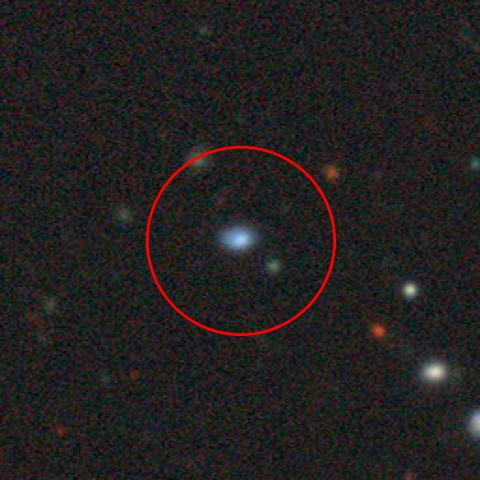
\includegraphics[width=\textwidth]{proposatal_candidatas_1/UCG03.jpg}
        \caption{UCG03}
    \end{subfigure}
    \begin{subfigure}[b]{0.22\textwidth}
        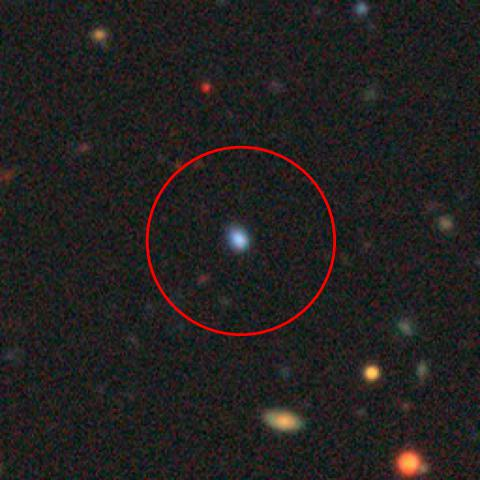
\includegraphics[width=\textwidth]{proposatal_candidatas_1/UCG04.jpg}
        \caption{UCG04}
    \end{subfigure}
    \begin{subfigure}[b]{0.22\textwidth}
        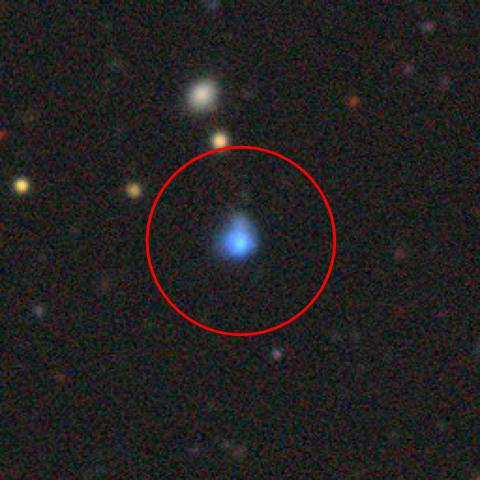
\includegraphics[width=\textwidth]{proposatal_candidatas_1/UCG05.jpg}
        \caption{UCG05}
    \end{subfigure}
    \begin{subfigure}[b]{0.22\textwidth}
        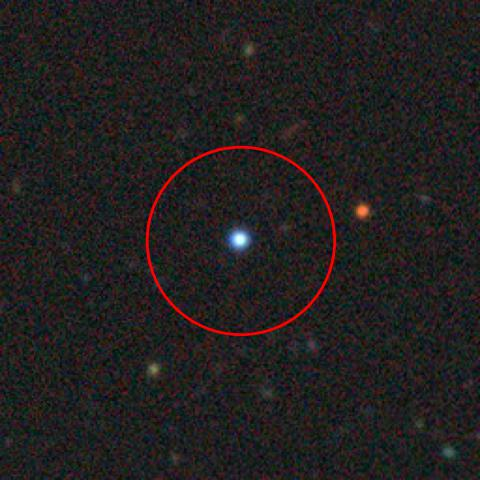
\includegraphics[width=\textwidth]{proposatal_candidatas_1/UCG06.jpg}
        \caption{UCG06}
    \end{subfigure}
    \begin{subfigure}[b]{0.22\textwidth}
        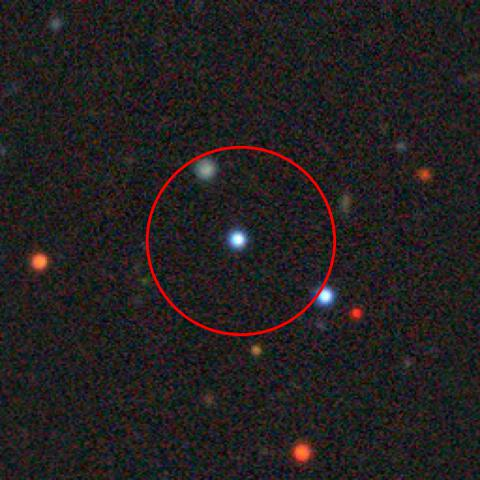
\includegraphics[width=\textwidth]{proposatal_candidatas_1/UCG07.jpg}
        \caption{UCG07}
    \end{subfigure}
    \begin{subfigure}[b]{0.22\textwidth}
        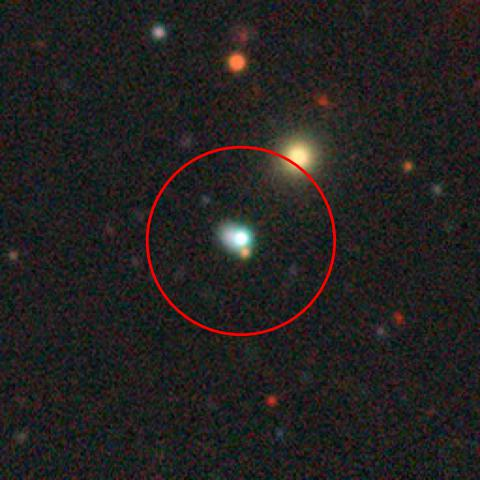
\includegraphics[width=\textwidth]{proposatal_candidatas_1/UCG08.jpg}
        \caption{UCG08}
    \end{subfigure}
    \begin{subfigure}[b]{0.22\textwidth}
        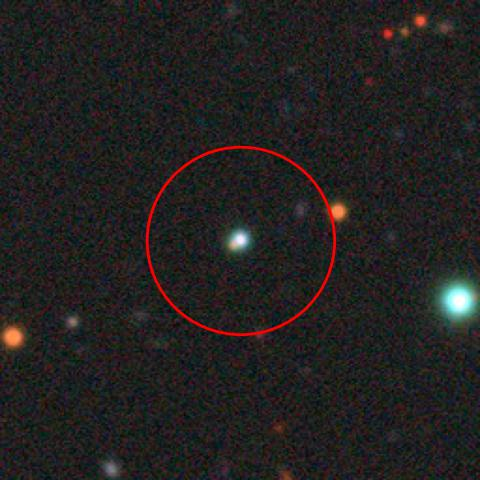
\includegraphics[width=\textwidth]{proposatal_candidatas_1/UCG09.jpg}
        \caption{UCG09}
    \end{subfigure}
    \begin{subfigure}[b]{0.22\textwidth}
        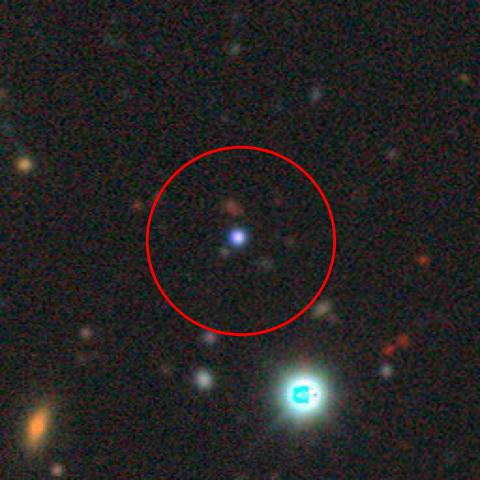
\includegraphics[width=\textwidth]{proposatal_candidatas_1/UCG10.jpg}
        \caption{UCG10}
    \end{subfigure}
    \begin{subfigure}[b]{0.22\textwidth}
        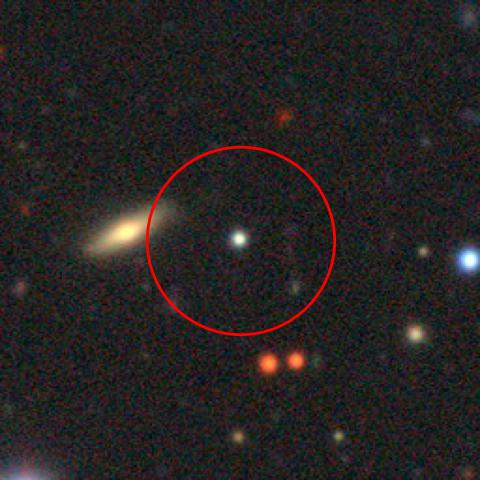
\includegraphics[width=\textwidth]{proposatal_candidatas_1/UCG11.jpg}
        \caption{UCG11}
    \end{subfigure}
    \begin{subfigure}[b]{0.22\textwidth}
        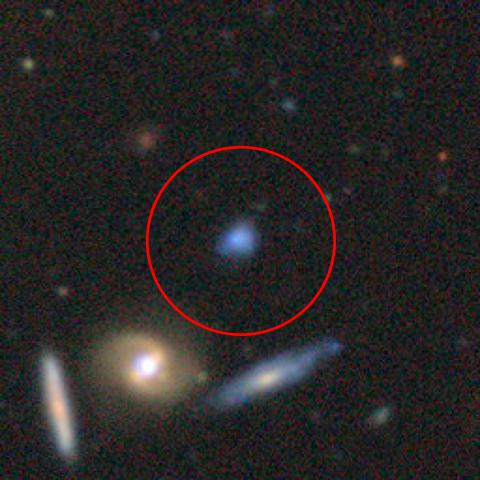
\includegraphics[width=\textwidth]{proposatal_candidatas_1/UCG12.jpg}
        \caption{UCG12}
    \end{subfigure}
    \begin{subfigure}[b]{0.22\textwidth}
        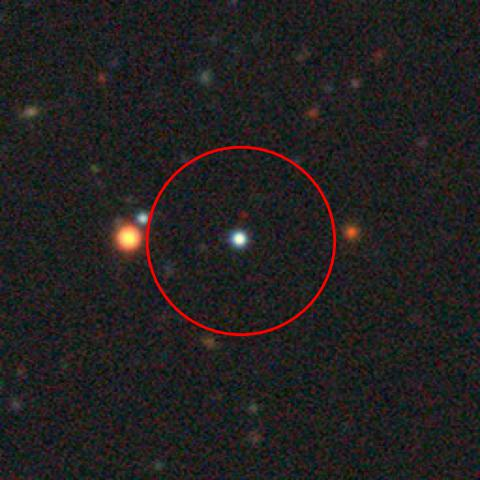
\includegraphics[width=\textwidth]{proposatal_candidatas_1/UCG13.jpg}
        \caption{UCG13}
    \end{subfigure}
    \begin{subfigure}[b]{0.22\textwidth}
        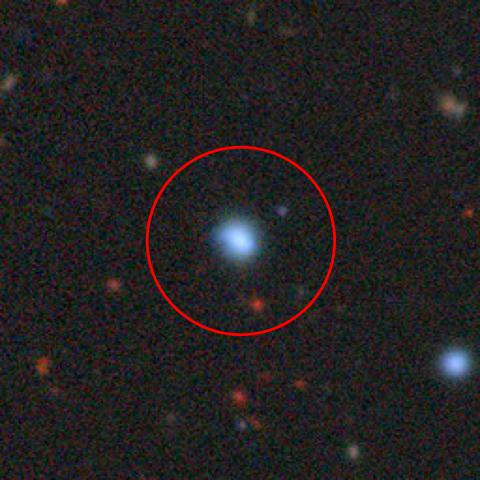
\includegraphics[width=\textwidth]{proposatal_candidatas_1/UCG14.jpg}
        \caption{UCG14}
    \end{subfigure}
    \begin{subfigure}[b]{0.22\textwidth}
        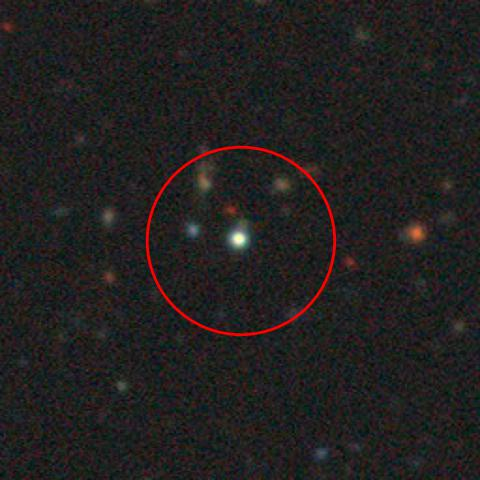
\includegraphics[width=\textwidth]{proposatal_candidatas_1/UCG15.jpg}
        \caption{UCG15}
    \end{subfigure}
    \begin{subfigure}[b]{0.22\textwidth}
        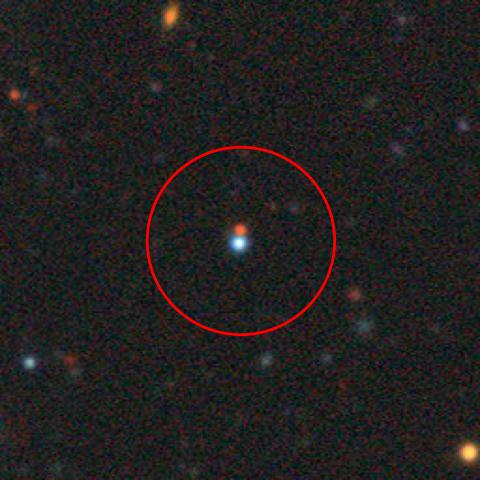
\includegraphics[width=\textwidth]{proposatal_candidatas_1/UCG16.jpg}
        \caption{UCG16}
    \end{subfigure}
    \begin{subfigure}[b]{0.22\textwidth}
        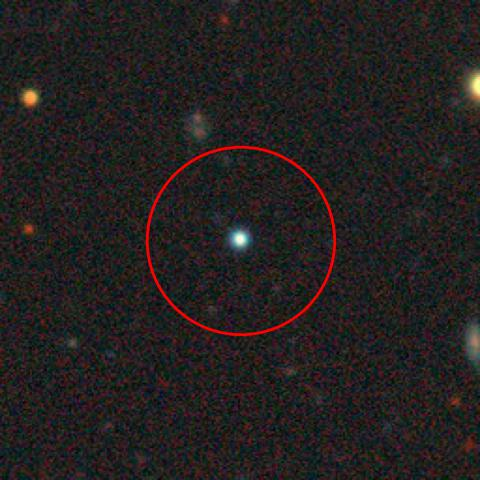
\includegraphics[width=\textwidth]{proposatal_candidatas_1/UCG17.jpg}
        \caption{UCG17}
    \end{subfigure}
    \begin{subfigure}[b]{0.22\textwidth}
        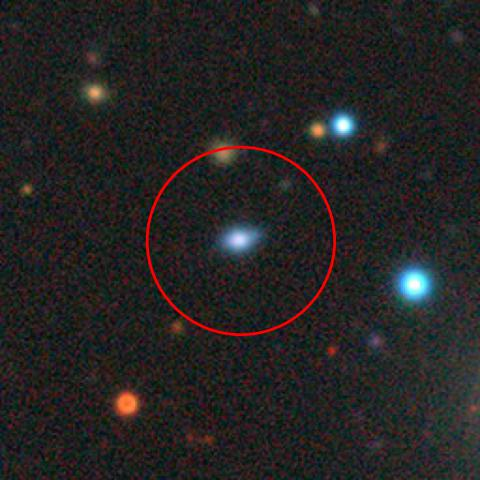
\includegraphics[width=\textwidth]{proposatal_candidatas_1/UCG18.jpg}
        \caption{UCG18}
    \end{subfigure}
    \caption{Imagens das candidatas a UCDs observadas com o GMOS no telescópio Gemini Sul, selecionadas de um projeto anterior. Imagens obtidas pelo Legacy Survey. Os nomes são os da Tabela \ref{candidatas_espectroscopia_1}.}
    \label{candidatas_espectroscopia_1_img}
\end{figure}

\section{Observações com o Gemini Sul}\label{sec:observacoes_gemini}
O Observatório Gemini é uma instalação astronômica internacional composta por dois telescópios gêmeos: um localizado no hemisfério norte, no Havaí, e outro no hemisfério sul, no Chile. O Gemini South, situado no Chile, é equipado com um espelho primário de 8,1 metros de diâmetro (assim como o Gemini North).

Para buscar novas galáxias ultracompactas no aglomerado de Fornax utilizamos dados espectroscópicos obtidos com o \ac{GMOS-S}, instalado no telescópio Gemini South, operando no modo de fenda longa. Essa abordagem permitiu obter espectros individuais de cada objeto.

Os dados espectroscópicos foram coletados através do repositório online do Gemini Observatory\footnote{Gemini Observatory, \textit{Gemini Observatory Archive}, disponível em \url{https://archive.gemini.edu}}.

As configurações utilizadas para as observações foram as seguintes:

\begin{itemize}
    \item \textbf{Modo de Observação}: Fenda longa (\textit{long-slit}).
    \item \textbf{Grating}: B600-G5303, com comprimento de onda central $\lambda_c = 550 \, \text{nm}$.
    \item \textbf{Largura da Fenda}: 1,5".
    \item \textbf{Resolução Espectral}: $R \sim 570$, considerando a largura da fenda escolhida.
    \item \textbf{Intervalo Espectral}: 4000\,\text{Å} a 7000\,\text{Å}, cobrindo desde o azul até quase o vermelho.
    \item \textbf{Tempo de Exposição por Objeto}: 1200 segundos, divididos em 3 exposições de 400 segundos cada.
    \item \textbf{Condições de Observação}: IQ=ANY, CC=80\%, WV=ANY, SB=ANY.
    \item \textbf{Razão Sinal-Ruído (S/N) Desejada}: Mínimo de 5 no espectro combinado (equivalente a S/N $\sim$ 3 por pixel espectral) no contínuo, suficiente para detectar o declive do contínuo azul e as principais linhas de absorção.
\end{itemize}

Dos 18 objetos dessa amostra, 14 foram observados com sucesso. Da Tabela \ref{candidatas_espectroscopia_1} não foram observadas as candidatas UCG04, UCG09, UCG11, e UCG17.

\section{Redução}\label{sec:reducao}
A redução dos dados espectroscópicos é uma etapa crucial para garantir a qualidade e a precisão das análises subsequentes. Essa etapa envolve a correção de artefatos instrumentais, a calibração de fluxos e a extração de espectros unidimensionais.

Os dados espectroscópicos do telescópio Gemini não passam por um tratamento inicial, então é necessário um pré-processamento. Esse passo é limpa as imagens de sinais indesejados, removendo ruídos dos instrumentos e convertendo os espectros bidimensionais em unidimensionais para análise.

Fizemos a redução dos dados usando o Software de Redução de Dados DRAGONS (Data Reduction for Astronomy with Gemini Observatory's Node System) \cite{dragons_python}. Esse software permite reduzir os dados tanto pela linha de comando quanto por meio de uma API em Python. Optamos pela API em Python para tornar o processo mais eficiente e agilizar a geração dos espectros unidimensionais (1D).

\textbf{Seleção de Dados}

O primeiro passo para a redução é a seleção dos dados que serão usados, como os arquivos de \textit{bias}, \textit{flats}, \textit{arcs}, estrelas padrão (\textit{standard star}) e os dados científicos. Utilizamos a função \verb|dataselect.select_data|, que permite filtrar os arquivos por algumas características específicas, como o tipo de detector e o objeto observado.

\textbf{Redução do \textit{Bias}}

A etapa inicial da redução é a correção de \textit{bias}, onde os arquivos são processados para remover o sinal eletrônico residual presente nas imagens. Utilizando a função \verb|Reduce|, criamos dois conjuntos de arquivos de \textit{bias}: um para as estrelas padrão e outro para os dados científicos. Essa correção visa garantir que o sinal obtido nas observações não seja contaminado por ruídos instrumentais.

\textbf{Redução dos \textit{Flats}}

Após a correção de \textit{bias}, processamos as imagens de \textit{flat-field}, que corrigem variações na resposta do detector em diferentes regiões do campo de visão. Os arquivos de \textit{flats} são selecionados e processados novamente com a função \verb|Reduce|, assegurando a uniformidade na resposta do detector em todas as partes do espectro.

\textbf{Redução dos \textit{Arcs}}

Na sequência, realizamos a redução dos arquivos de \textit{arcs}, que contêm linhas de emissão conhecidas utilizadas para calibrar a escala de comprimento de onda dos espectros. A função \verb|Reduce| é aplicada para processar os \textit{arcs}, ajustando as linhas de emissão observadas ao modelo teórico e garantindo que os comprimentos de onda sejam medidos com precisão.

\textbf{Redução da Estrela Padrão}

Para a redução da estrela padrão (\textit{standard star}), também utilizamos a função \verb|Reduce| para processar essas observações, gerando um espectro calibrado em fluxo, que serve como referência para a normalização dos espectros dos objetos científicos. O espectro resultante é plotado e analisado para verificar a qualidade da calibração.

\textbf{Redução dos Dados Científicos}

Finalmente, os dados científicos são reduzidos aplicando todas as correções anteriores (\textit{bias}, \textit{flat}, \textit{arc}) aos dados da observação dos objetos de interesse, novamente utilizando a função \verb|Reduce|. Esse processo resulta na geração dos espectros unidimensionais (\textit{1D}) que poderão ser analisados.

\section{Resultados}\label{sec:resultados}
Realizamos a análise dos espectros para identificar as características dos objetos observados. Usamos o programa PYRAF, uma linguagem de comando para IRAF baseada na linguagem de script Python.

Com os espectros brutos reduzidos pelo DRAGONS, antes de qualquer análise, precisamos limpar os dados de ruídos e remover sinais indesejados. Primeiro, removemos possíveis linhas de céu e raios cósmicos, que afetam nossos espectros. 

Observamos a presença de linhas e picos no espectro que não estão associados a nenhuma emissão ou absorção conhecida, associados aos resíduos de subtração de linhas do céu. Esses picos apresentam uma amplitude significativamente maior do que o restante do espectro e necessitam ser eliminados. Geralmente, eles surgem após transições abruptas de subida e descida, ao contrário das emissões ou absorções genuínas, que tendem a ter uma aparência mais gaussiana.

Em cada um dos espectros, são eliminados os artefatos mais óbvios, resultando em espectros limpos e com uma escala de visualização que facilita a identificação de linhas de interesse.

Após processar todos os espectros dos objetos observados e realizar a limpeza necessária, procedemos à análise das possíveis linhas de emissão ou absorção para estimar. A detecção de redshifts extremamente baixos é indicativa da proximidade do objeto dentro da Via Láctea. Vamos considerar como galáxias apenas objetos com $z > 0.002$, já que objetos com redshifts menores são geralmente estrelas da Via Láctea.

Redshifts podem ser obtidos de linhas de absorção e de linhas de emissão. Linhas de absorção resultam da absorção de luz pelas camadas exteriores da atmosfera estelar.

Linhas de emissão indicam a presença de gás ionizado no objeto. Tais linhas estão comumente associadas a processos de formação estelar recente, em que regiões de gás interestelar são ionizadas por estrelas jovens e quentes, ou à atividade nuclear, onde são formadas em discos de acreção em torno de buracos negros supermassivos situados no centro das galáxias.

% Para a análise das linhas, podemos usar como base alguns espectros de diferentes objetos observados pelo Sloan Digital Sky Survey (SDSS). Na Figura \ref{sdds_espectro}, mostramos alguns exemplos de espectros de alguns tipos de galáxias vindos do SDSS.

% \begin{figure}[!ht]
%     \begin{center}
%     % \setcaptionmargin{1cm}
%     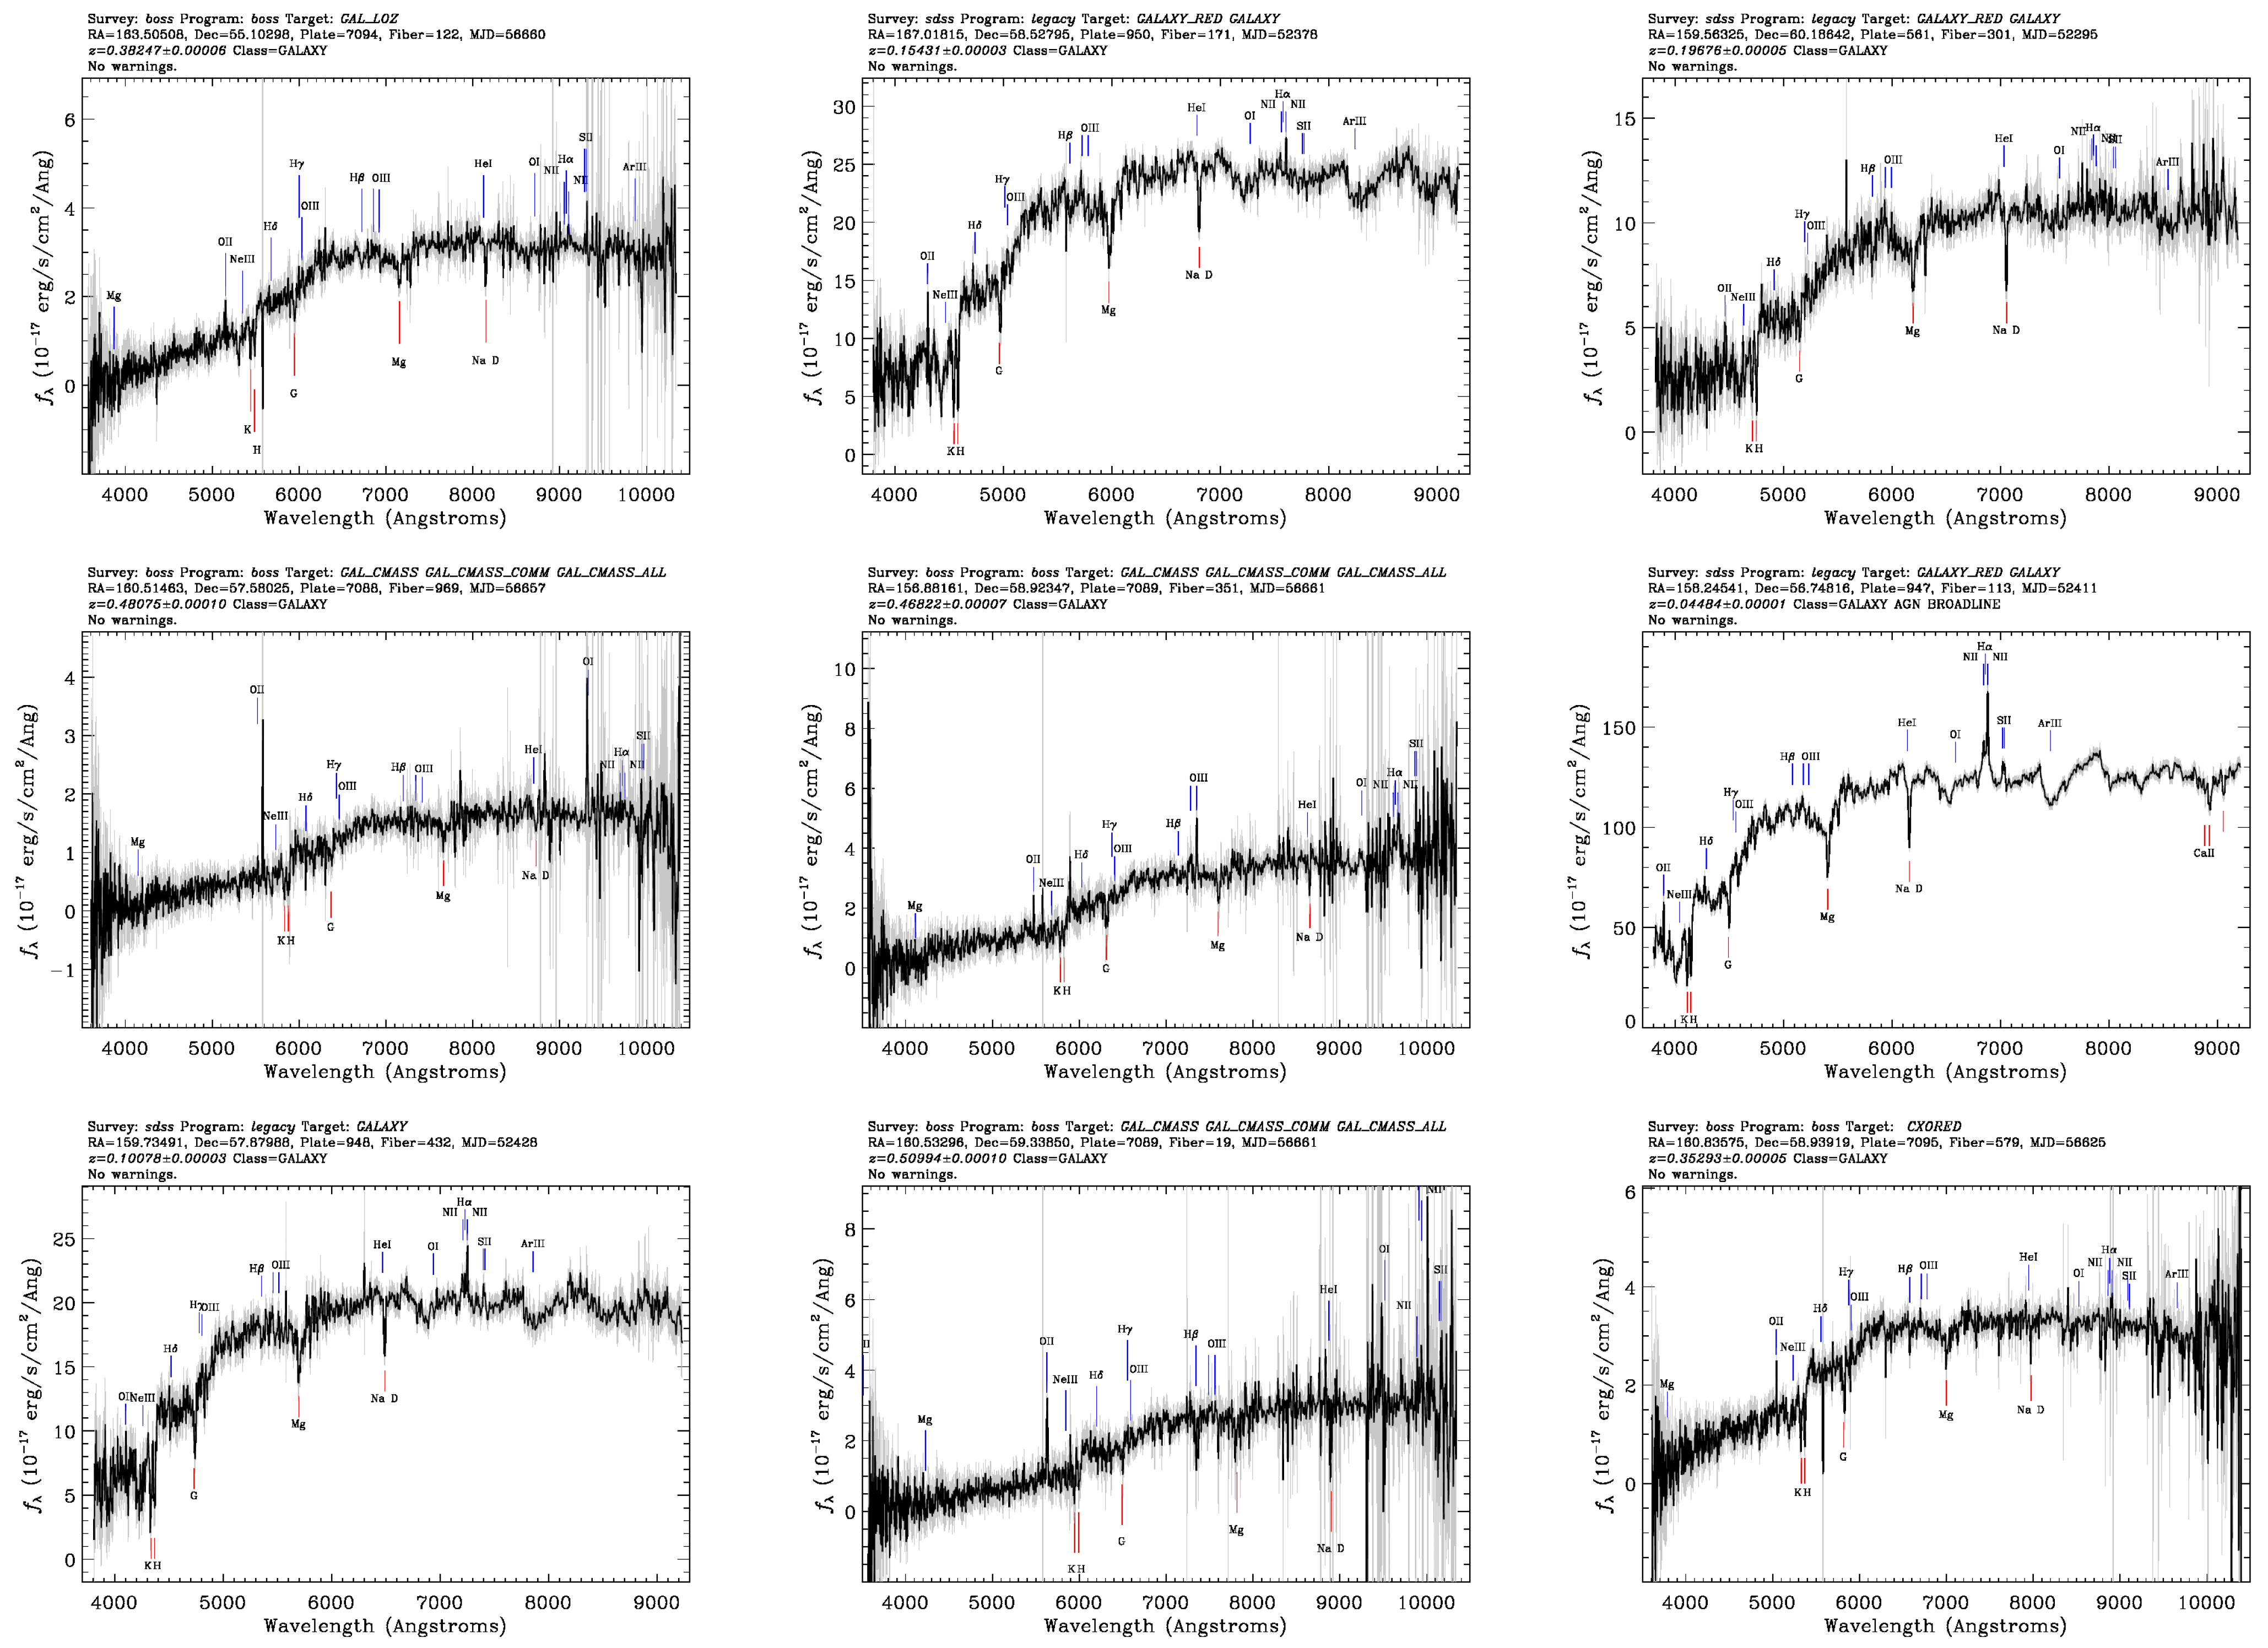
\includegraphics[width=1\columnwidth,angle=0]{espectros/sdds_espectro_01.png}
%     \caption[]{Espectros de exemplo do SDSS de diferentes classes de objetos.}
%     \label{sdds_espectro}
%     \end{center}
% \end{figure}    

Os espectros, depois de limparmos os artefatos para análise, são apresentados no conjunto das Figuras \ref{espectros_candidatas_1_p1} e \ref{espectros_candidatas_1_p2}.

\begin{figure}[H]
    \centering
    \captionsetup{justification=centering}
    \begin{subfigure}[b]{0.45\textwidth}
        \includegraphics[width=\textwidth]{espectros/UCG01.png}
        \caption{UCG01}
    \end{subfigure}
    \begin{subfigure}[b]{0.45\textwidth}
        \includegraphics[width=\textwidth]{espectros/UCG02.png}
        \caption{UCG02}
    \end{subfigure}
    \begin{subfigure}[b]{0.45\textwidth}
        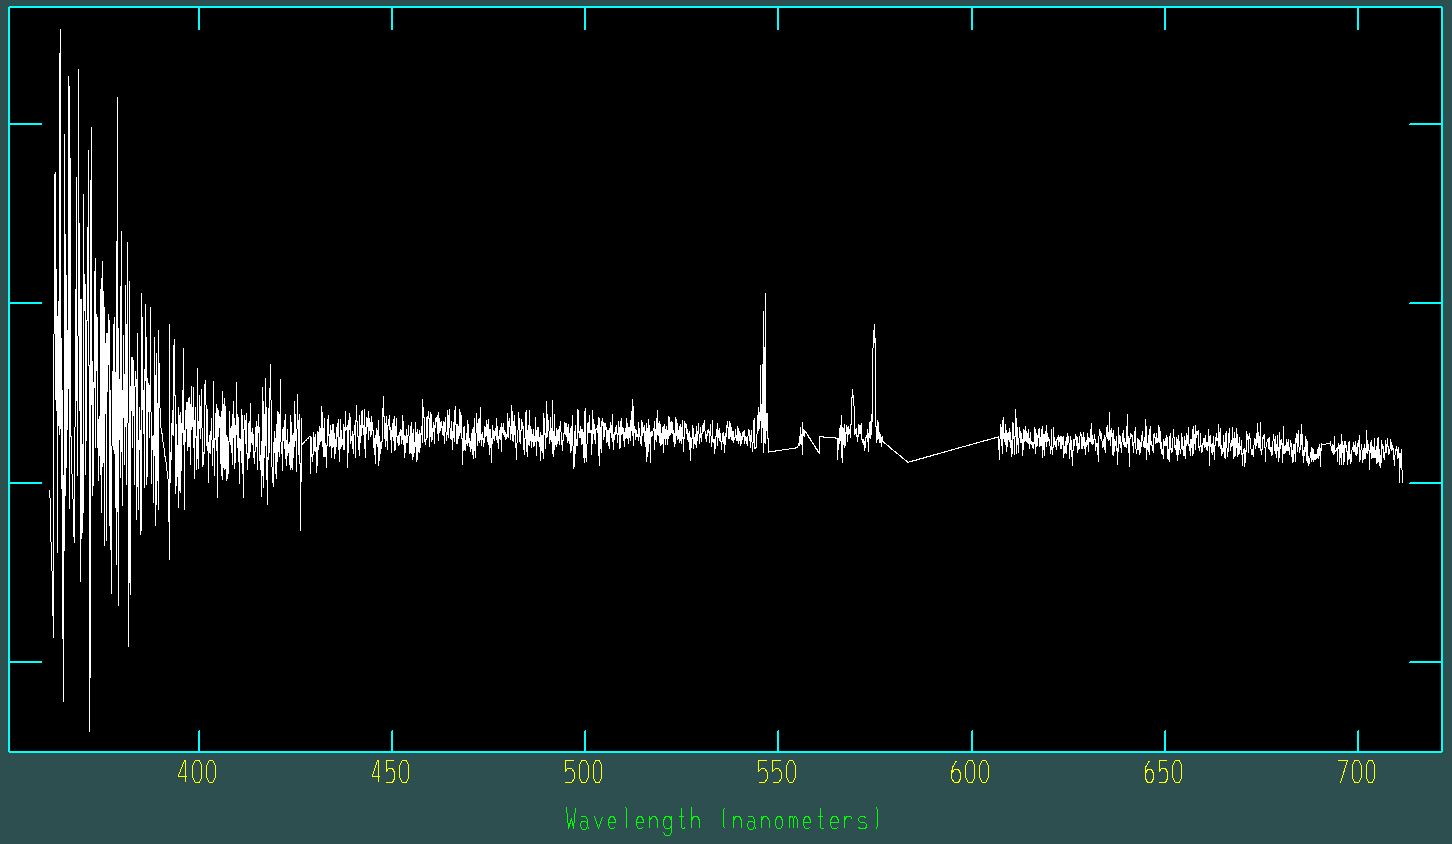
\includegraphics[width=\textwidth]{espectros/UCG03.png}
        \caption{UCG03}
    \end{subfigure}
    \begin{subfigure}[b]{0.45\textwidth}
        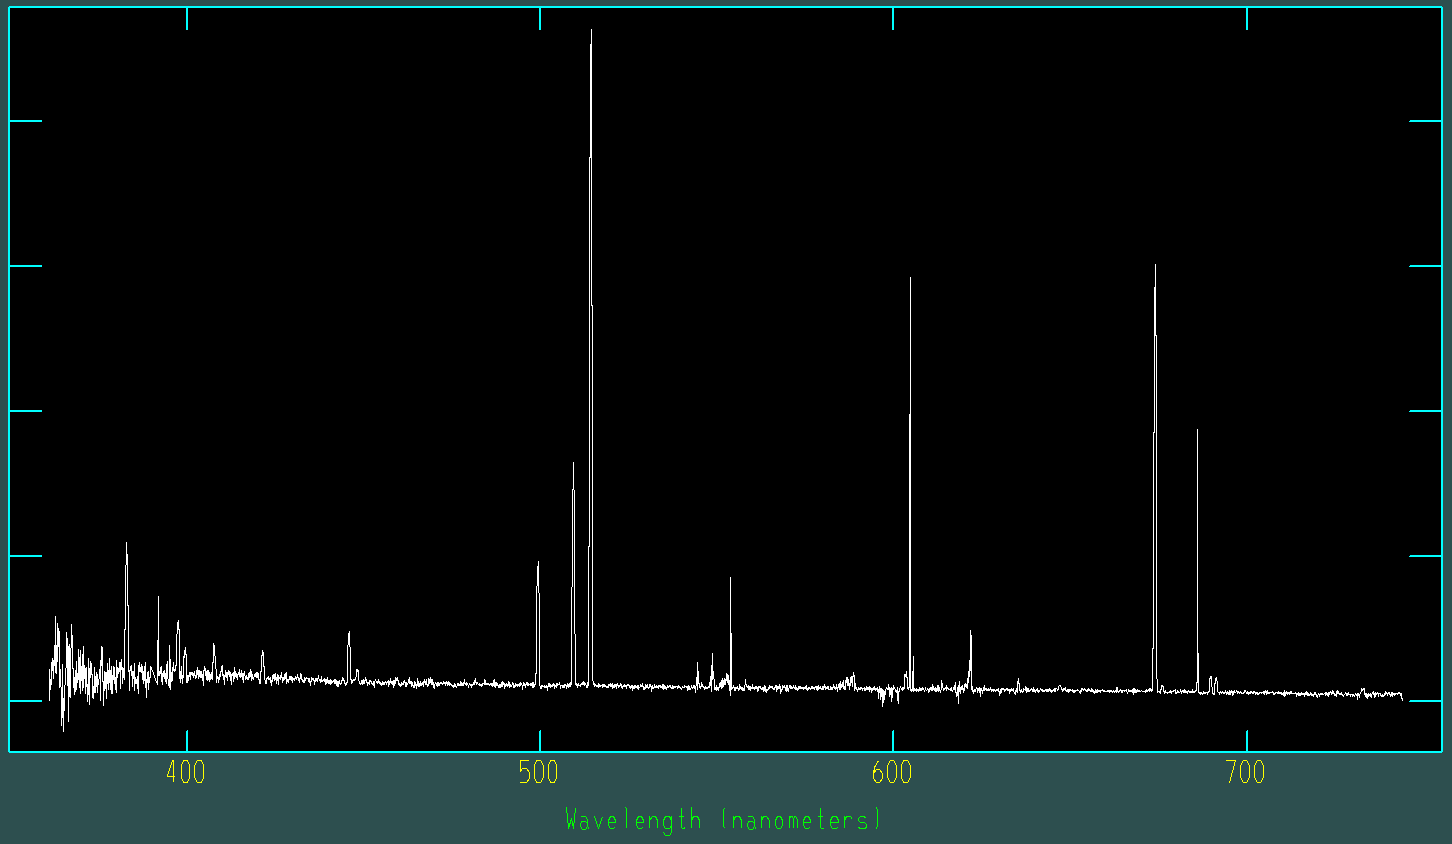
\includegraphics[width=\textwidth]{espectros/UCG05.png}
        \caption{UCG05}
    \end{subfigure}
    \begin{subfigure}[b]{0.45\textwidth}
        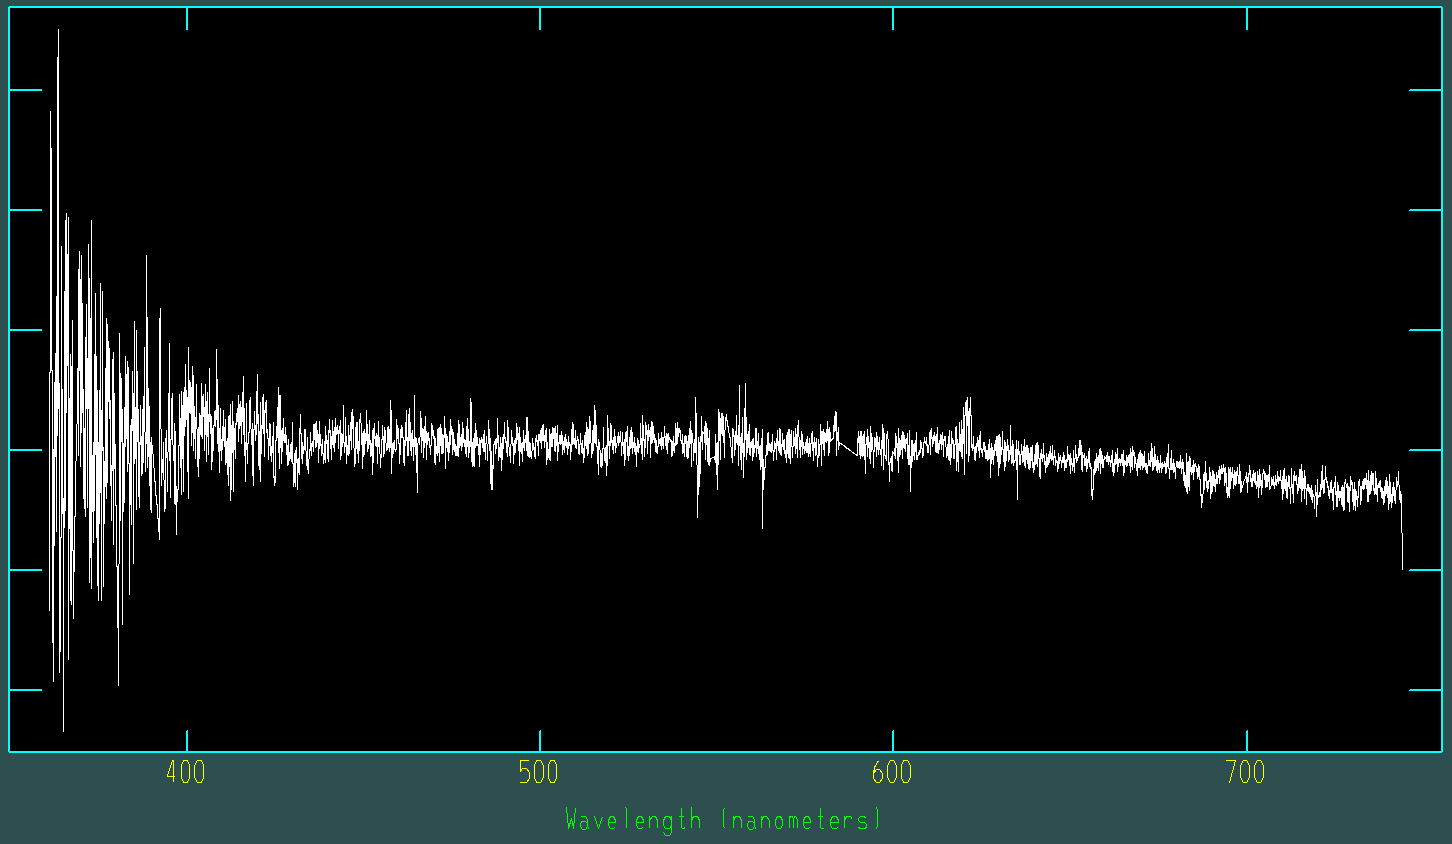
\includegraphics[width=\textwidth]{espectros/UCG06.png}
        \caption{UCG06}
    \end{subfigure}
    \begin{subfigure}[b]{0.45\textwidth}
        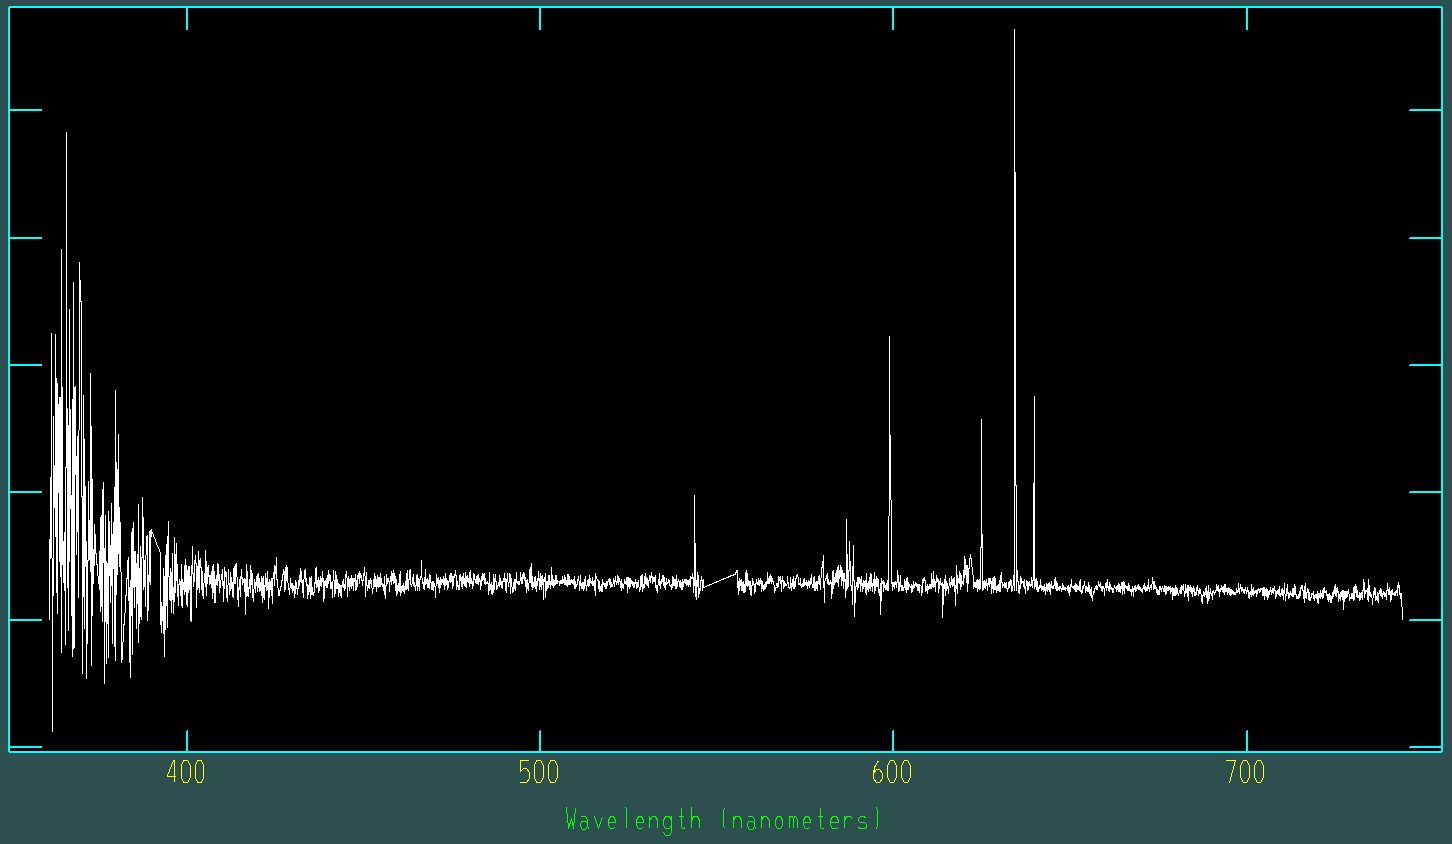
\includegraphics[width=\textwidth]{espectros/UCG07.png}
        \caption{UCG07}
    \end{subfigure}
    \begin{subfigure}[b]{0.45\textwidth}
        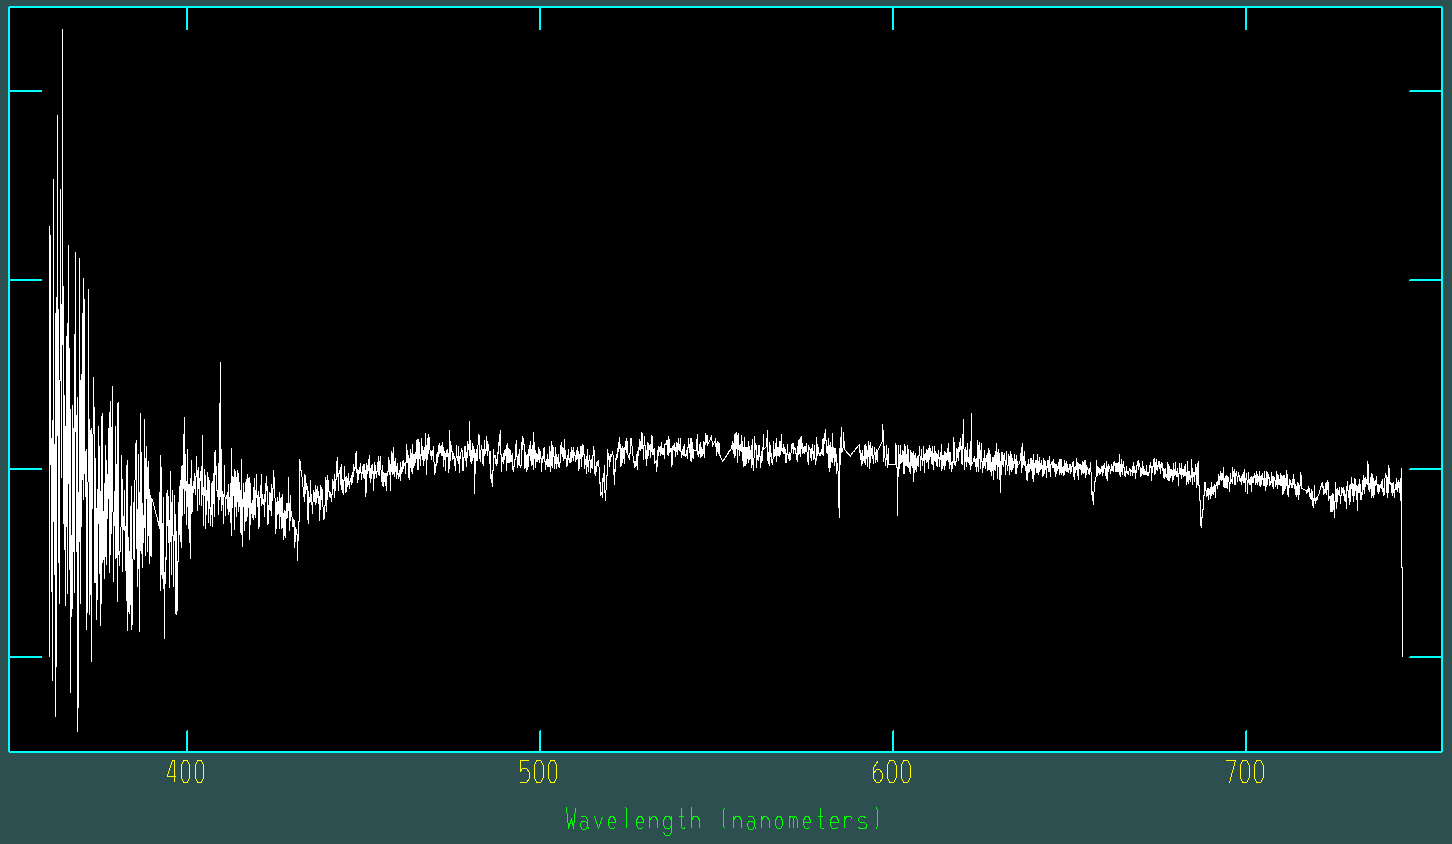
\includegraphics[width=\textwidth]{espectros/UCG08.png}
        \caption{UCG08}
    \end{subfigure}
    \begin{subfigure}[b]{0.45\textwidth}
        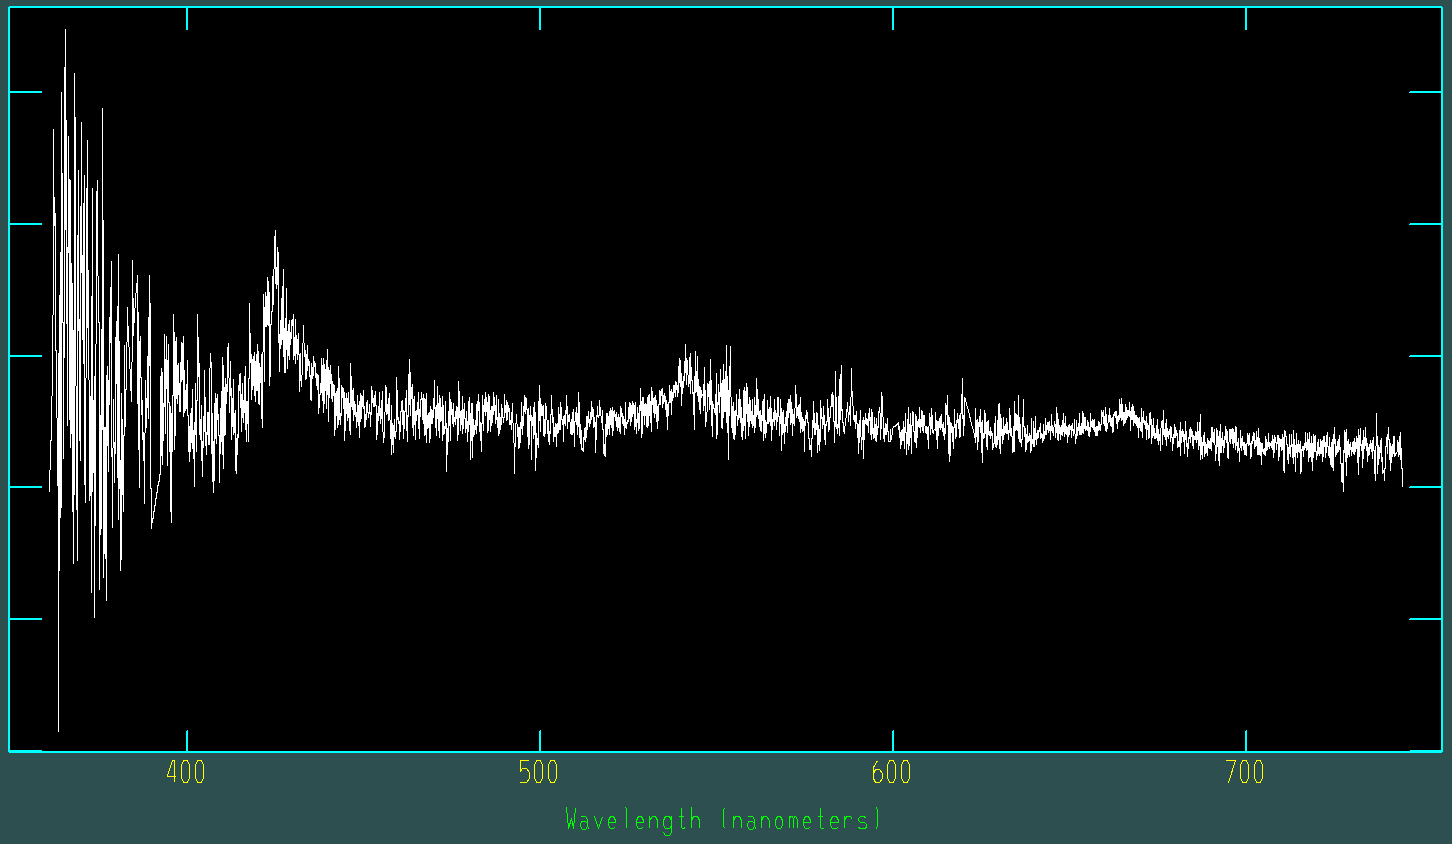
\includegraphics[width=\textwidth]{espectros/UCG10.png}
        \caption{UCG010}
    \end{subfigure}
    \caption{Espectros das candidatas a UCDs (Candidatas 1 até 10) do primeiro pedido de tempo observadas no Gemini Sul. Os nomes \textit{UCG} correspondem ao nome interno usado para o pedido de tempo de observação.}
    \label{espectros_candidatas_1_p1}
\end{figure}


\begin{figure}[H]
    \centering
    \begin{subfigure}[b]{0.45\textwidth}
        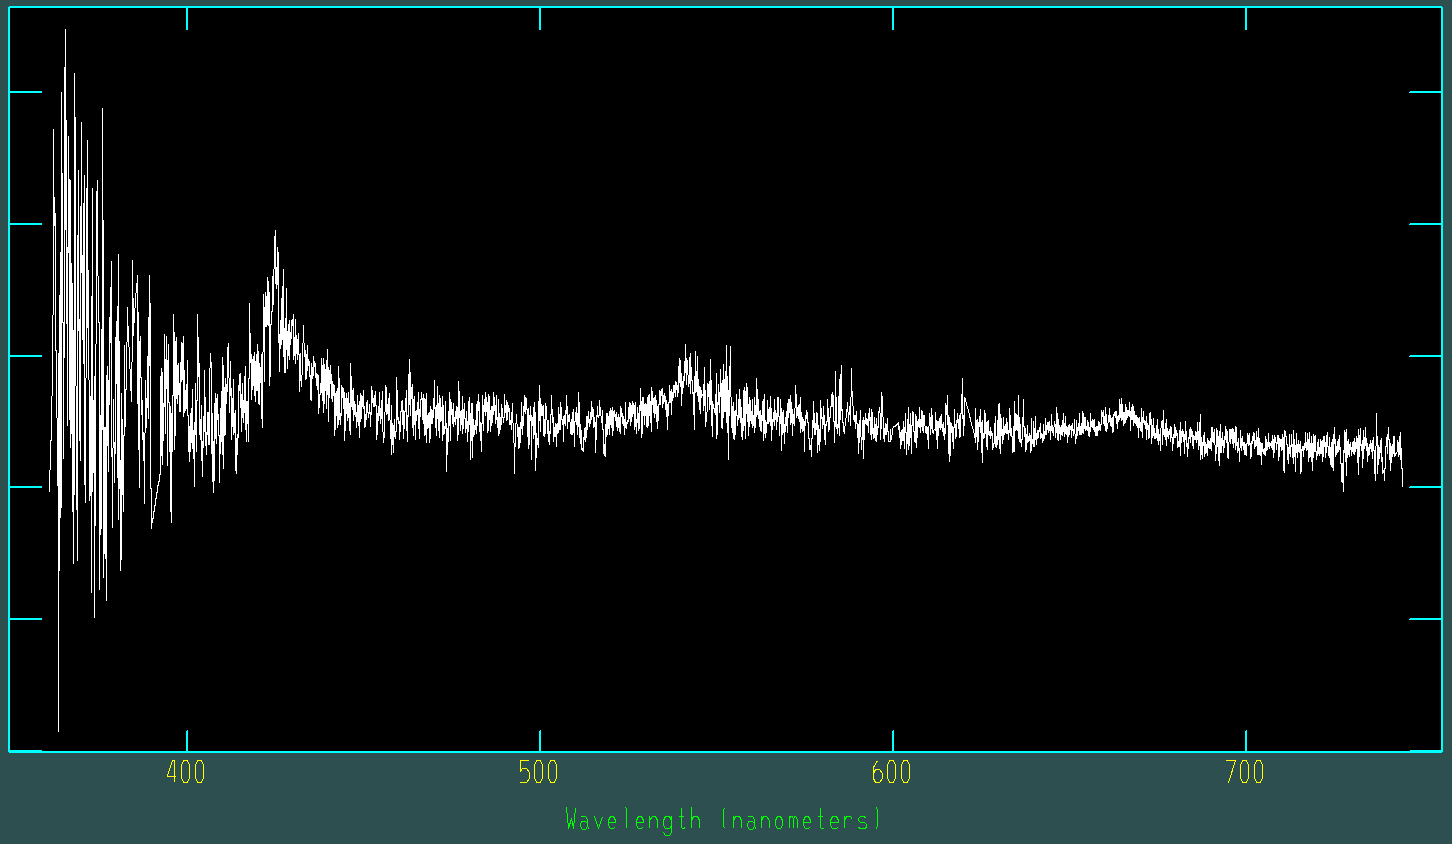
\includegraphics[width=\textwidth]{espectros/UCG10.png}
        \caption{UCG10}
    \end{subfigure}
    \begin{subfigure}[b]{0.45\textwidth}
        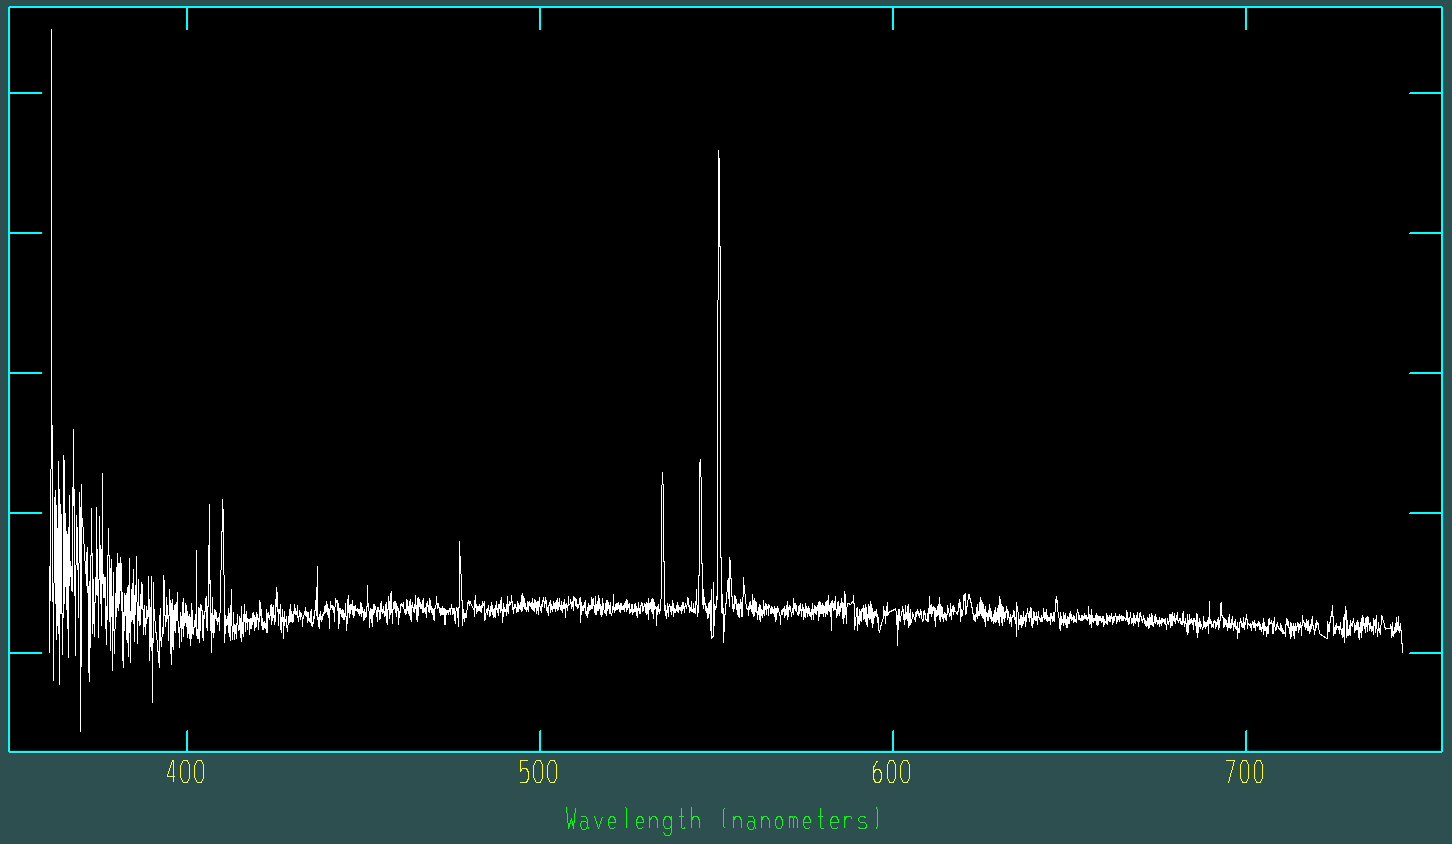
\includegraphics[width=\textwidth]{espectros/UCG12.png}
        \caption{UCG12}
    \end{subfigure}
    \begin{subfigure}[b]{0.45\textwidth}
        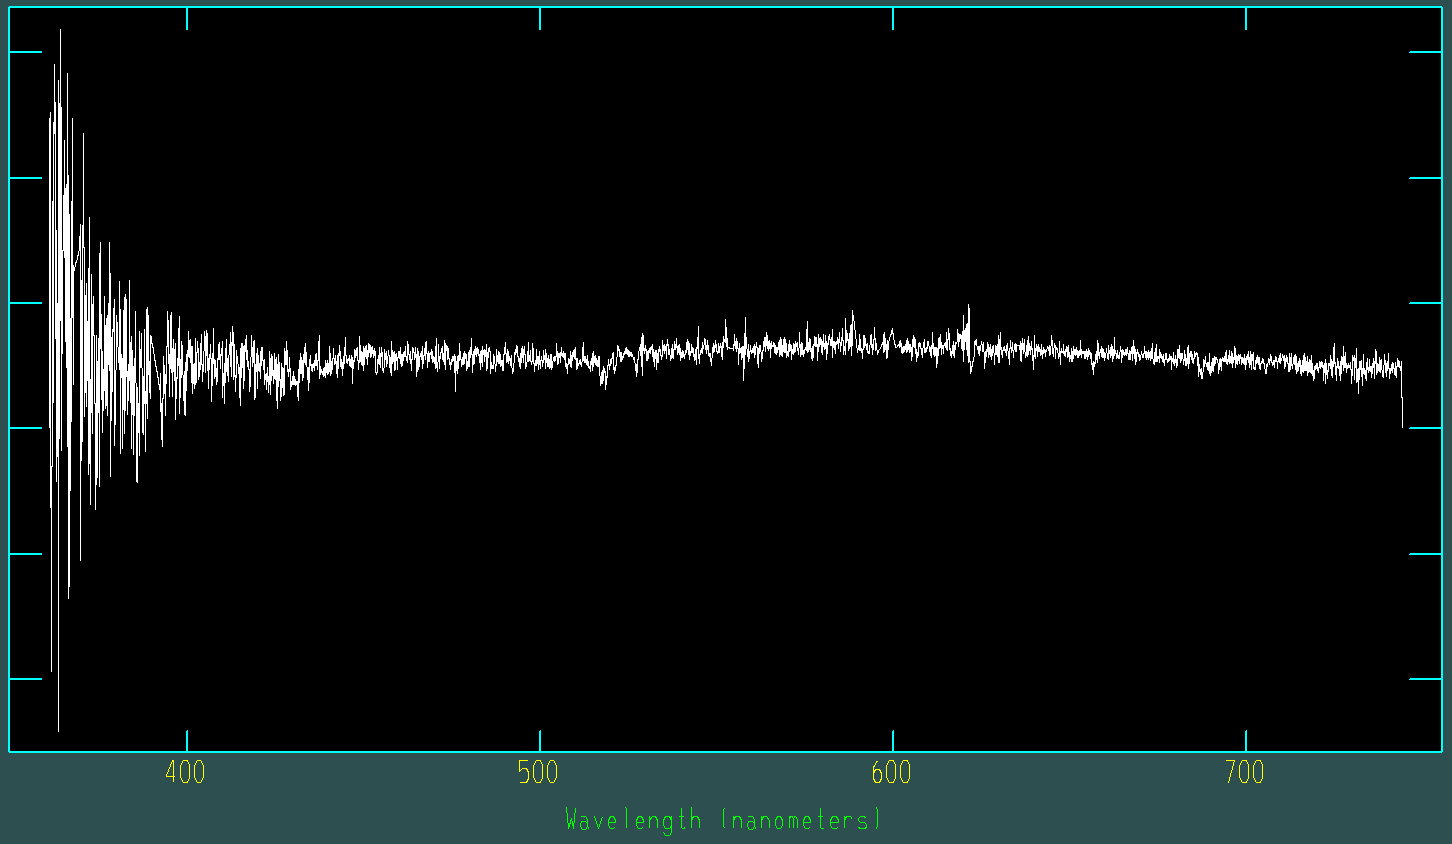
\includegraphics[width=\textwidth]{espectros/UCG13.png}
        \caption{UCG13}
    \end{subfigure}
    \begin{subfigure}[b]{0.45\textwidth}
        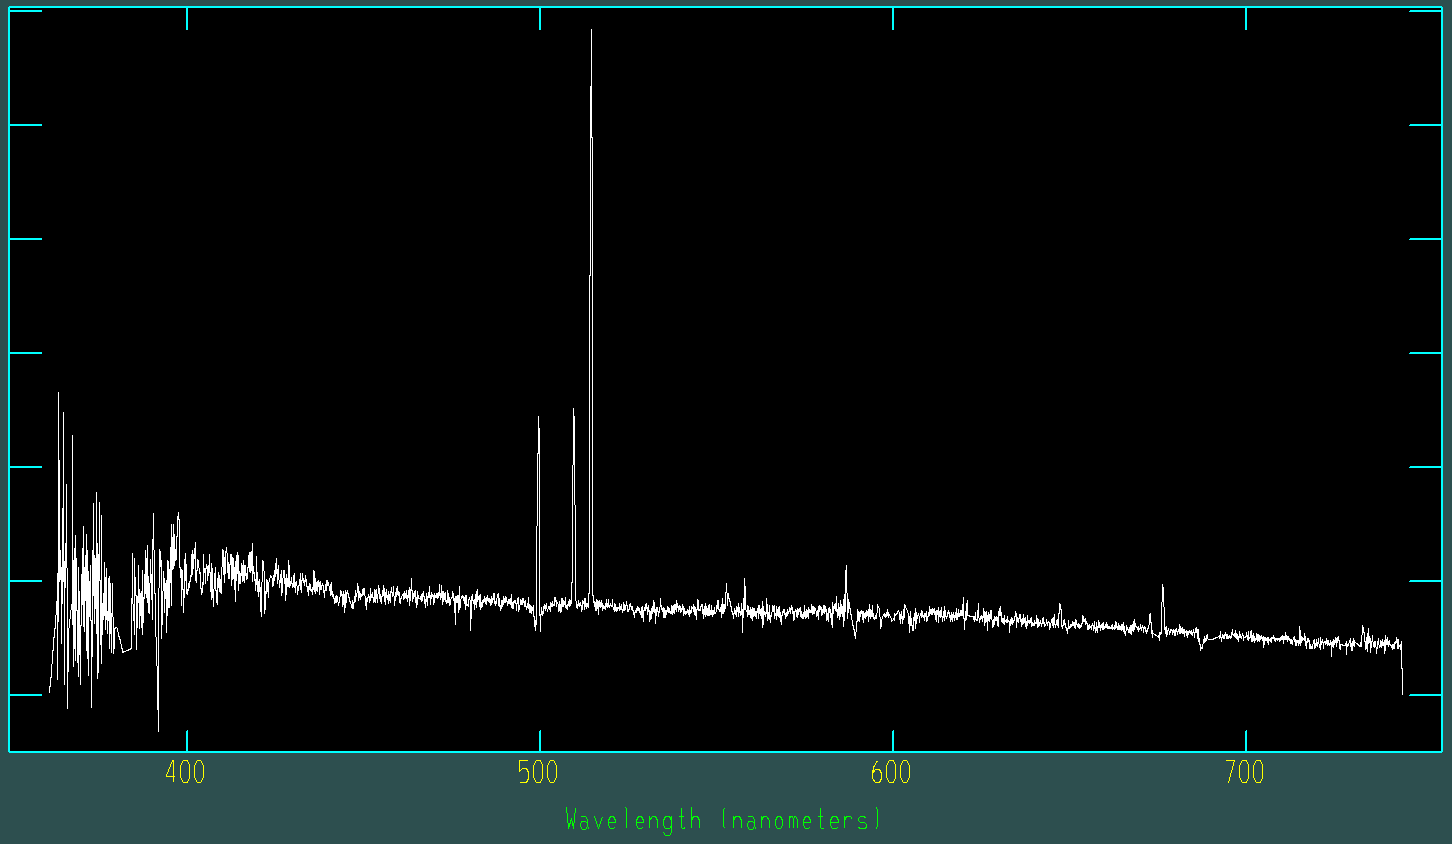
\includegraphics[width=\textwidth]{espectros/UCG14.png}
        \caption{UCG14}
    \end{subfigure}
    \begin{subfigure}[b]{0.45\textwidth}
        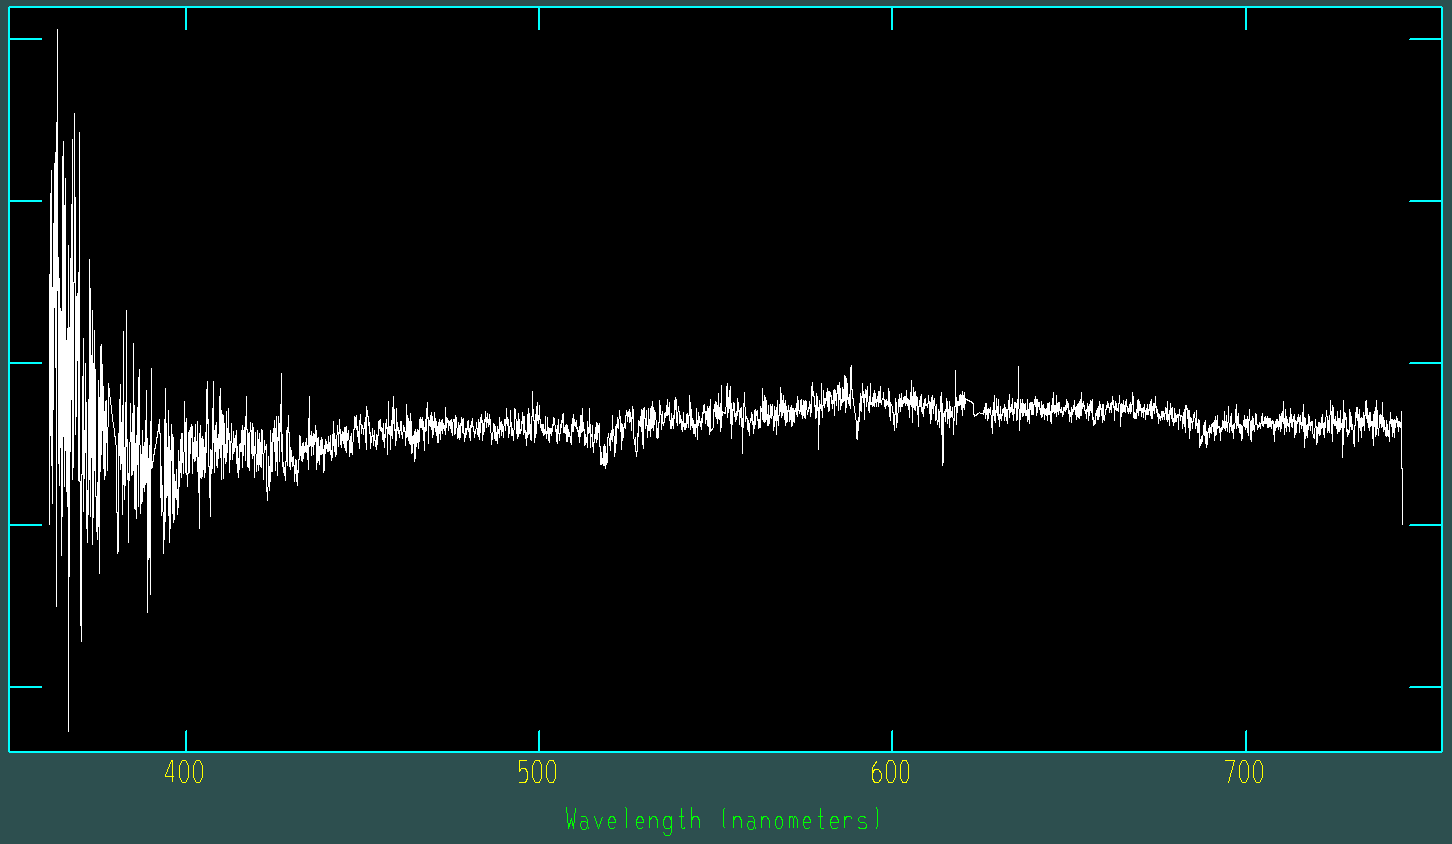
\includegraphics[width=\textwidth]{espectros/UCG15.png}
        \caption{UCG15}
    \end{subfigure}
    \begin{subfigure}[b]{0.45\textwidth}
        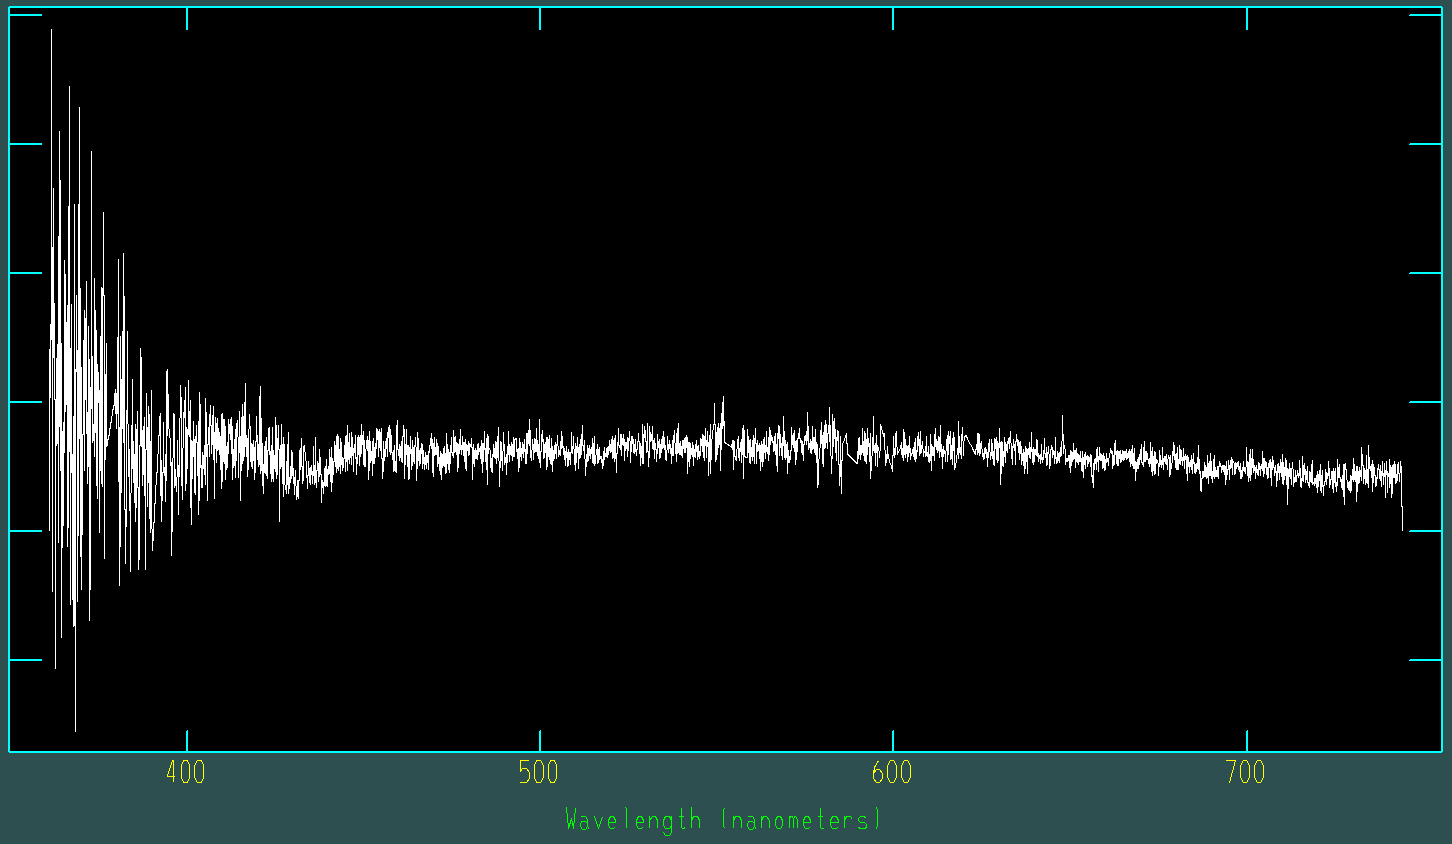
\includegraphics[width=\textwidth]{espectros/UCG16.png}
        \caption{UCG16}
    \end{subfigure}
    \begin{subfigure}[b]{0.45\textwidth}
        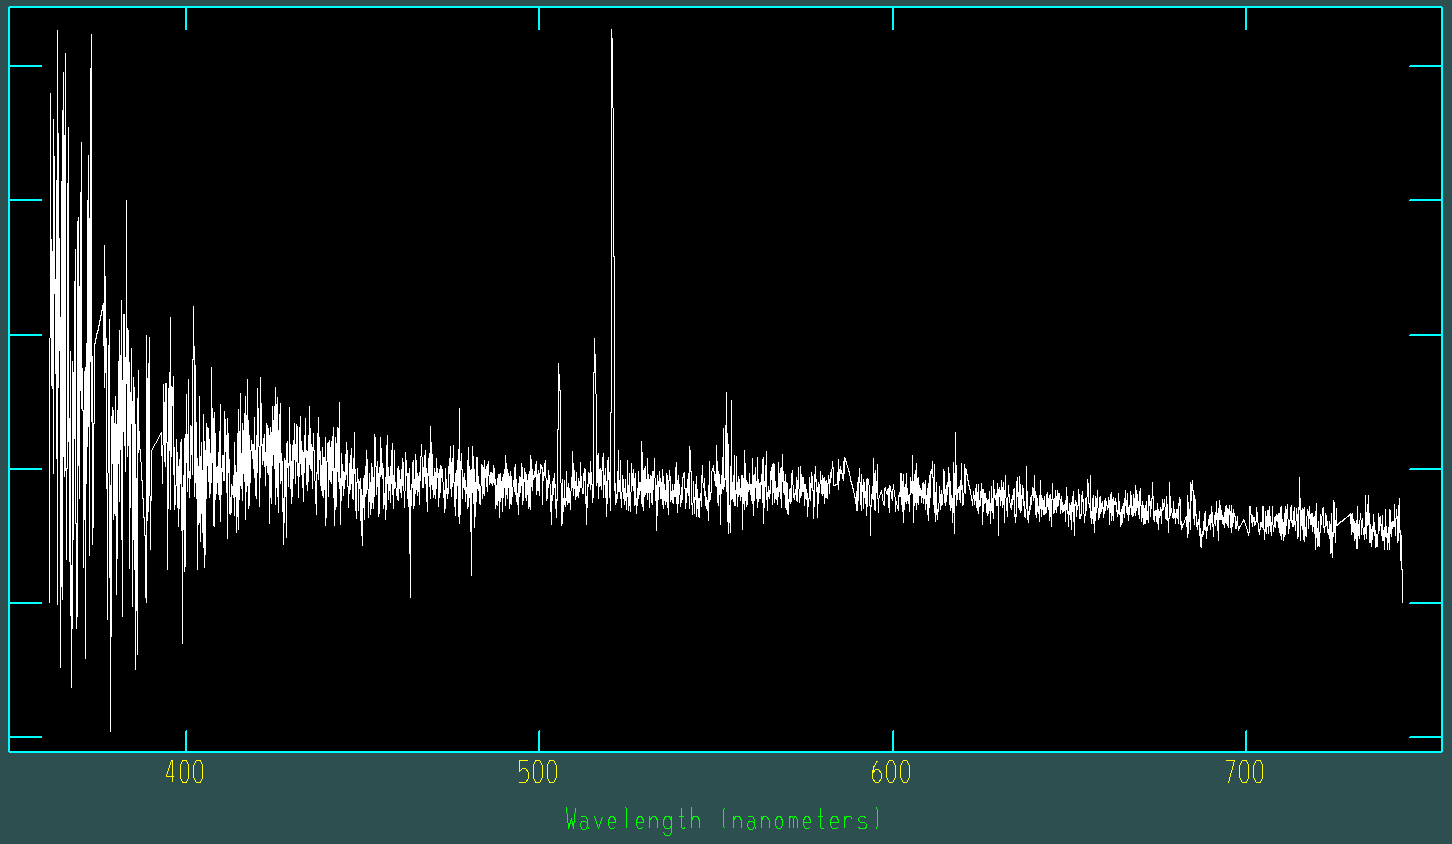
\includegraphics[width=\textwidth]{espectros/UCG18.png}
        \caption{UCG18}
    \end{subfigure}
    \caption{Espectros das candidatas a UCDs (Candidatas 10 até 18) do primeiro pedido de tempo observadas no Gemini Sul. Os nomes \textit{UCG} correspondem ao nome interno usado para o pedido de tempo de observação.}
    \label{espectros_candidatas_1_p2}
\end{figure}

Na Tabela \ref{redshift_candidatas_1}, apresentamos os redshifts obtidos para cada objeto, após a identificação de pelo menos duas linhas e o deslocamento em relação ao repouso.


\begin{table}[!ht]
    \centering
    \caption{Redshifts (\textit{z}) obtidos a partir dos espectros do conjunto de candidatas a UCDs observadas com o GMOS no telescópio Gemini Sul, selecionadas de um projeto anterior. A coluna $OBJ_{name}$ é o nome interno da candidata utilizado no pedido de tempo do Gemini.} 
    \begin{tabular}{lcc}
        \toprule
        $OBJ_{name}$ & z   \\
        \midrule
        UCG01     & 0.0005 \\
        UCG02     & 0.0004 \\
        UCG03     & 0.147 \\
        UCG05     & 0.02 \\
        UCG06     & -0.0003 \\
        UCG07     & -0.0003 \\
        UCG08     & -0.0001 \\
        UCG10     & 2.48 \\
        UCG12     & 0.0995 \\
        UCG13     & 0.0004 \\
        UCG14     & 0.027 \\
        UCG15     & 0.0006 \\
        UCG16     & 0.0004 \\
        UCG18     & 0.039 \\
        \bottomrule
    \end{tabular}
    \label{redshift_candidatas_1}
\end{table}


Ao final da análise, foram obtidos 14 espectros (UCG01, UCG02, UCG03, UCG05, UCG06, UCG07, UCG08, UCG10, UCG12, UCG13, UCG14, UCG15, UCG16, UCG18).

Temos 9 classificados como estrelas (UCG01, UCG02, UCG06, UCG07, UCG08, UCG13, UCG15, UCG16), 1 como quasar (UCG10) e 5 como galáxias (UCG03, UCG05, UCG12, UCG14, UCG18). Das galáxias encontradas nessa amostra, nenhuma foi classificada como pertencente ao aglomerado de Fornax.

Essa análise inicial de algumas candidatas, ainda que não tenha dado os resultados esperados, foi importante para o início do projeto. Em especial, ajudou no aprendizado da análise dos espectros e na redução dos dados.






